
In order to choose the best working conditions for a group of people, it is necessary to establish, whether the climate of a particular place plays any part in determining an individual's productivity.

The first aspect of a climate that we are going to be examining is its temperature. A number of studies \cite{Taylor2015,Muller2012} have shown, that temperature does, in fact, have a considerable impact on human cognitive functions. One scientific paper in particular, however, has shown to be an invaluable source, when it comes to determining the extent of this impact. A NBER working paper from 2013 \cite{Chetty2013} has studied the correlation, between productivity and indoor temperature (Figure \ref{temp:research}). This research presents us with several important observations. Firstly, the ideal temperature for mental work is around $22\degree C$. We can also use the data measured in this study in order to estimate the function to determine the productivity of a person working at a given temperature.

\begin{figure}[ht]
    \centering
        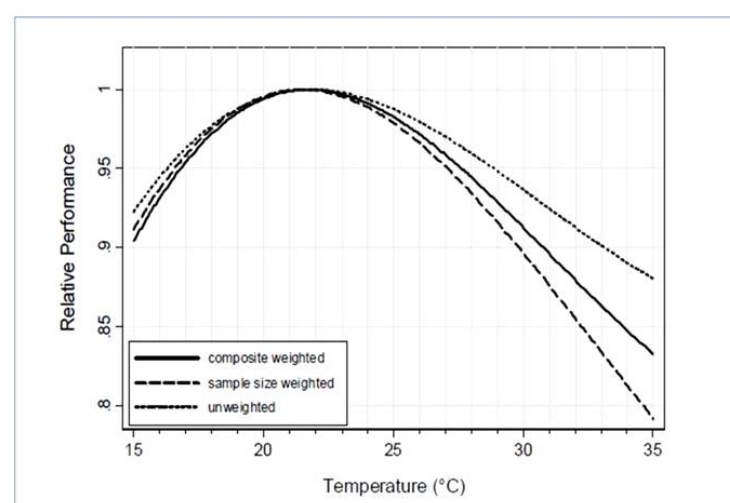
\includegraphics[width=0.6\textwidth]{graph_temp}
    \caption{Task performance vs. temperature \cite{Chetty2013}}
    \label{temp:research}
\end{figure}

Using the least-squares fit we arrived at an approximation of (Figure \ref{temp:approximation}):

$$P\approx -1.06907 \cdot 10^{-7} \cdot t^{4}+0.00003 \cdot t^{3}-0.00344 \cdot t^{2}+0.11109 \cdot t-0.08269$$

\noindent where $t$ is the temperature of the destination.

\begin{figure}[ht]
    \centering
        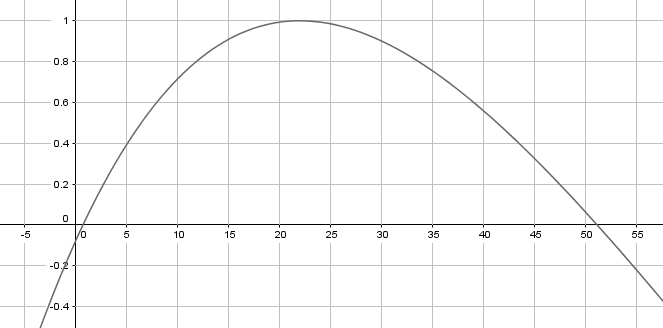
\includegraphics[width=0.4\textwidth]{graph4}
    \caption{Task performance vs. temperature, function fit}
    \label{temp:approximation}
\end{figure}

It is pretty effortless to obtain some data upon which temperature impact can be estimated. We used historical temperature data per month derived from the Climate Research Unit (Mitchell et al, 2003), aggregated by countries.

This approach does, however, have its shortcomings. The first problem we have to consider is that the original research only studied the effects of indoor temperature. In our case, the indoor temperature is not so dependent on a particular city, since it can be easily controlled by heating or air conditioning. We can, however, predict, that outside temperature is going to have an effect on productivity, whether it be by decreasing comfort while traveling, or in case the outside temperature cannot be entirely differentiated from the indoor one, because of insufficient heating, insulation etc. We therefore decided to model the relationship between productivity and outside temperature based on the model for indoor temperature, since we can safely assume that both models behave similarly. To estimate an individual's productivity, in this case, we will use the function mentioned above, using a parameter, that will determine the magnitude of performance impact.

$$P=\left( (-1.06907 \cdot 10^{-7} \cdot t^{4}+0.00003 \cdot t^{3}-0.00344 \cdot t^{2}+0.11109 \cdot t-0.08269)-1 \right)\cdot K_{T}+1$$

\noindent where $K_{T}$ is the temperature effect parameter. For the purposes of this model, we estimate this value to be around:
$$K_{T}\approx 0.05$$
It is also worth noting, that according to our research, no considerable adaptation to local temperature can occur in such a short period of time. Our model considers the effect of temperature to stay the same throughout the meeting.

This simple approach, however, may not be precise for large countries where the temperatures significantly differ for different locations within the country. Further improvement of the approach could be made by obtaining more precise data not aggregated by countries.

Additionally, the month of the day with appropriate day index $D$ is used to determine the average temperature in the country for the given day of the meeting. An enhancement could base the temperature prediction not only on the month but also on the day of a month and the average temperatures in the previous and following months.
